% Generated by AP Math GOLD PILOT deterministic Python generator.
% input id: H03_axis_tangent_circles
\documentclass{article}
\usepackage[margin=1cm]{geometry}
\def\pgfsysdriver{pgfsys-dvisvgm.def}
\usepackage{fontspec}
\setmainfont{Malgun Gothic}
\setsansfont{Malgun Gothic}
\usepackage{amsmath}
\usepackage{amssymb}
\usepackage{pgfplots}
\pgfplotsset{compat=1.18}
\pagestyle{empty}
\begin{document}
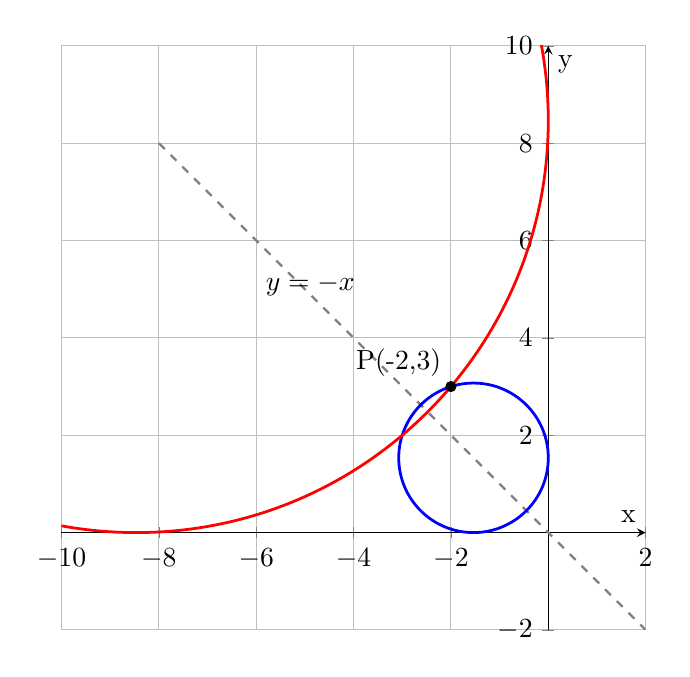
\begin{tikzpicture}
\begin{axis}[width=13cm,height=9cm,axis equal image,axis lines=middle,grid=major,xmin=-10,xmax=2,ymin=-2,ymax=10,xlabel={x},ylabel={y},clip=true]
\addplot[gray, dashed, line width=0.8pt] coordinates {(-8,8) (-7.875,7.875) (-7.75,7.75) (-7.625,7.625) (-7.5,7.5) (-7.375,7.375) (-7.25,7.25) (-7.125,7.125) (-7,7) (-6.875,6.875) (-6.75,6.75) (-6.625,6.625) (-6.5,6.5) (-6.375,6.375) (-6.25,6.25) (-6.125,6.125) (-6,6) (-5.875,5.875) (-5.75,5.75) (-5.625,5.625) (-5.5,5.5) (-5.375,5.375) (-5.25,5.25) (-5.125,5.125) (-5,5) (-4.875,4.875) (-4.75,4.75) (-4.625,4.625) (-4.5,4.5) (-4.375,4.375) (-4.25,4.25) (-4.125,4.125) (-4,4) (-3.875,3.875) (-3.75,3.75) (-3.625,3.625) (-3.5,3.5) (-3.375,3.375) (-3.25,3.25) (-3.125,3.125) (-3,3) (-2.875,2.875) (-2.75,2.75) (-2.625,2.625) (-2.5,2.5) (-2.375,2.375) (-2.25,2.25) (-2.125,2.125) (-2,2) (-1.875,1.875) (-1.75,1.75) (-1.625,1.625) (-1.5,1.5) (-1.375,1.375) (-1.25,1.25) (-1.125,1.125) (-1,1) (-0.875,0.875) (-0.75,0.75) (-0.625,0.625) (-0.5,0.5) (-0.375,0.375) (-0.25,0.25) (-0.125,0.125) (0,0) (0.125,-0.125) (0.25,-0.25) (0.375,-0.375) (0.5,-0.5) (0.625,-0.625) (0.75,-0.75) (0.875,-0.875) (1,-1) (1.125,-1.125) (1.25,-1.25) (1.375,-1.375) (1.5,-1.5) (1.625,-1.625) (1.75,-1.75) (1.875,-1.875) (2,-2)};
\draw[blue, solid, line width=1pt] (axis cs:-1.535898,1.535898) circle [radius=1.535898];
\draw[red, solid, line width=1pt] (axis cs:-8.464102,8.464102) circle [radius=8.464102];
\addplot[only marks,mark=*,mark size=1.8pt,black] coordinates {(-2,3)};
\node[anchor=south east] at (axis cs:-2,3) {P(-2,3)};
\node[anchor=north west] at (axis cs:-6,5.5) {$y=-x$};
\end{axis}
\end{tikzpicture}
\end{document}
